\section{JavaScript} \label{chapter_javascript}

JavaScript is the programming language used for scripting in HTML documents. Code written in JavaScript resides in the script block of the HTML Domain Object Model (DOM), as seen in figure \ref{fig:htmldom}. This language's purpose is amongst others to allow dynamic reload of content on events, like clicks, to reduce bandwidth and allow user interactions. Input can also be verified and the document's design can be altered. These operations can be done by manipulating the DOM tree, yet arbitrary computations can also be done. JavaScript is a just-in-time compiled language.

\begin{figure}[htp]
  \begin{center}
    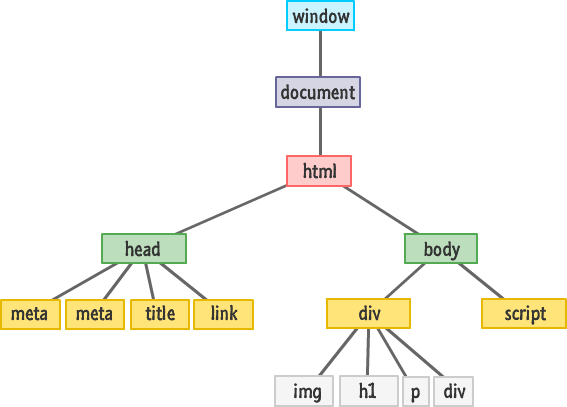
\includegraphics[width=0.9\columnwidth]{resources/html_dom.png}
  \end{center}
  \caption{HTML Domain Object Model [kirupa.com]}
  \label{fig:htmldom}
\end{figure}


\subsection{Type System}

When looking at arbitrary computations, it is important to note the key characteristics of JavaScript's type system:

\begin{itemize}

\item \textit{Dynamically typed}. Types of objects are resolved at runtime; static checks are not done. This means operations like late binding or downcasting are performed during execution. This allows developers to write code faster, but operations might fail at runtime due to e.g. missing operators.

\item \textit{Object-oriented}. As noted before, JavaScript utilizes objects. It is important to note that even CPU native types, like a 32 bit integer, are wrapped into JavaScript primitive type objects. While this simplifies development by adding utility functions, addtitional overhead occurs during runtime.

\item \textit{Classless}. Objects are not instantiations of pre-defined classes. They are defined as key-value pairs inside curly brackets, as seen in listing \ref{js_type}. This notation is refered to as the JavaScript Object Notation. (JSON) It allows arbitrary hierarchical nesting of data structures, like additional objects or arrays.

\item \textit{Prototypes}. As JavaScript is classless, prototypes are used. If multiple objects with the same members are desired, a prototype object is created and copied. These copies can again be arbitrarily modified.

\end{itemize}

\lstset{caption={JavaScript type system and JSON example},label=js_type}
\begin{lstlisting}[frame=single,basicstyle=\footnotesize]
var prototype = {
  "Publisher": "Xema",
  "ID": "1234-5678-9012-3456",
  "Owner": {
    "Name": "Max",
    "male": true,
    "Hobbys": ["Riding", "Golf"],
    "Age": 42,
  }
};

var copy = prototype;
copy["Currency"] = "EURO";
copy["Owner"]["Hobbys"].push("Reading");
\end{lstlisting}


\subsection{Memory Management}

JavaScript does not support explicit memory management. Functions like malloc or free, new or delete are not available. The web browser must provide a Garbage Collection mechanism. Its purpose is to automatically remove unused objects from memory. This makes development easier, as object ownership has not to be considered, and prevents memory leaks. Implementations in current web browsers are based on the mark-and-sweep algorithm. Basically, unreferenced, in the sense of unreachable, objects are to be removed. 

Applications though may suffer from badly timed garbage collecting. JavaScript and current web browsers provide no interface to control the time a garbage collection occurs. Today's implementations are highly optimized. Still, real-time and memory intensive applications, like many HPC applications, have to be implemented carefully. Creation of too many objects should be avoided and patterns benefiting garbage collection should be used. \cite{browsergc}
